\subsection{* Structure of complete regular Noetherian local rings}

In this section, we use definitions and results from Chapter IX.

Let A be a regular Noetherian complete local ring; denote by p the characteristic of its residue field \(\kappa_{A}\) , and distinguish two cases.

\begin{enumerate}
\def\labelenumi{\Alph{enumi})}
\tightlist
\item
  \(p = 0\) . Then (IX, § 3, n° 3, th. 1), there exists a subfield K of A such that the canonical projection of A onto \(\kappa_{\mathrm{A}}\) induces an isomorphism of K onto \(\kappa_{\mathrm{A}}\) . Applying then cor. 3 of th. 1 of n° 2 to the K-algebra A, we deduce:
\end{enumerate}

PROPOSITION 6. --- Let A be a regular Noetherian complete local ring, whose residue field \(\kappa_{\mathrm{A}}\) has characteristic 0. Set \(n = \dim(\mathrm{A})\) . Then A is isomorphic to the ring of formal power series \(\kappa_{\mathrm{A}}[[\mathrm{X}_{1}, ..., \mathrm{X}_{n}]]\) .

\begin{enumerate}
\def\labelenumi{\Alph{enumi})}
\setcounter{enumi}{1}
\tightlist
\item
  \(p \neq 0\) . A Cohen subring of A is any subring V of A which is a \(p\)-ring such that \(A = \mathfrak{m}_{A} + V\) (IX, § 2, no. 2, def. 2). The ring V is local; its maximal ideal \(\mathfrak{m}_{V}\) is generated by \(p \cdot 1_{V}\) ; consequently we have \(\mathfrak{m}_{A} \cap V = \mathfrak{m}_{V}\) and the canonical injection of V into A induces, by passing to the quotient, an isomorphism of fields \(\kappa_{V}\) onto \(\kappa_{A}\) . If \(p \cdot 1_{A} = 0\) , V is a field of characteristic \(p\) . Otherwise, V is a discrete valuation ring whose field of fractions has characteristic zero (IX, § 2, no. 1, cor. 1 to prop. 1). It is proved (IX, no. 2, th. 1) that A has Cohen subrings.
\end{enumerate}

Examples. --- 1) Let \(k\) be a field of characteristic \(p \neq 0\) and \(n\) be a positive integer. The ring of formal power series \(k[[X_1, ..., X_n]]\) is a complete regular local Noetherian ring, of dimension \(n\) and \(k\) is a Cohen subring of \(k[[X_1, ..., X_n]]\) .

\begin{enumerate}
\def\labelenumi{\arabic{enumi})}
\setcounter{enumi}{1}
\item
  Let V be a complete discrete valuation ring and n a positive integer. The ring of formal power series \(V_{n} = V[[X_{1}, ..., X_{n}]]\) is a complete regular local Noetherian ring, of dimension \(n + 1\) and V is a Cohen subring of \(V_{n}\) .
\item
  Keep the previous notation. A polynomial P in \(V_{n}[T]\) of degree \(d \geqslant 2\) is special if it is of the form \(T^{d} + \sum_{i=1}^{d} a_{i} T^{d-i}\) , where \(a_{1}, \ldots, a_{d-1}\) belong to \(m_{V_{n}}\) , \(a_{d}\) belongs to \(m_{V} + m_{V_{n}}^{2}\) but not to \(m_{V_{n}}^{2}\). In particular, P is an Eisenstein polynomial for \(m_{V_{n}}\) . Set A = \(V_{n}[T]/(P)\). By the corollary to Prop. 4 of No. 4, the ring A is a complete regular local Noetherian ring, of dimension \(n + 1\). If t is the class of T modulo (P), the sequence \((1, t, \ldots, t^{d-1})\) is a basis of the \(V_{n}\) -module A, and \((X_{1}, \ldots, X_{n}, t)\) is a coordinate system of A: indeed, there exists a uniformizer π of V such that \(a_{d} \equiv \pi \mod m_{V_{n}}^{2}\) ; since we also have
\end{enumerate}

\[
a _ {d} = - t \left(t ^ {d - 1} + a _ {1} t ^ {d - 2} + \dots + a _ {d - 1}\right),
\]

we have \(\pi\in\mathfrak{m}_{\mathrm{A}}^{2}\) ; since \(\mathfrak{m}_{\mathrm{A}}\) is generated by \(\{\pi,\mathrm{X}_{1},..., \mathrm{X}_{n},t\}\) , this proves our assertion. Moreover, V is a Cohen subring of A, since \(\kappa_{\mathrm{V}}\) is identified with \(\kappa_{\mathrm{V}_{n}}\) , and \(\kappa_{\mathrm{V}_{n}}\) is identified with \(\kappa_{\mathrm{A}}\) by the corollary to Prop. 4 of No. 4.

THEOREM 2. --- Let A be a complete regular Noetherian local ring whose residue field has characteristic ≠ 0, and let V be a Cohen subring of A. Set n = dim(A).

\begin{enumerate}
\def\labelenumi{\alph{enumi})}
\item
  Suppose that V is a field. Then the V-algebra A is isomorphic to the algebra of formal power series \(V[[X_{1}, ..., X_{n}]]\) .
\item
  Suppose that V is a complete discrete valuation ring and that one has \(m_{V} \not\subset m_{A}^{2}\) . Then, the V-algebra A is isomorphic to the algebra of formal power series \(V[[X_{1}, ..., X_{n-1}]]\) .
\item
  Suppose that V is a complete discrete valuation ring and that one has \(\mathfrak{m}_{\mathrm{V}} \subset \mathfrak{m}_{\mathrm{A}}^{2}\) . There then exists a special polynomial P in \(\mathrm{V}[[\mathrm{X}_{1}, ..., \mathrm{X}_{n-1}]]\) {[}T{]} and a V-isomorphism from A onto \(\mathrm{V}[[\mathrm{X}_{1}, ..., \mathrm{X}_{n-1}]]\) {[}T{]}/(P).
\end{enumerate}

Assertion a) follows immediately from cor. 3 of th. 1 of no. 2.

Let us prove \(b\). Let \((x_{1},\ldots,x_{m})\) be a sequence of elements of \(\mathfrak{m}_{\mathrm{A}}\), and let \(\varphi_{0}\) be the homomorphism from \(\mathrm{V}[\mathrm{X}_{1},\ldots,\mathrm{X}_{m}]\) to A which coincides with the identity on V and sends \(\mathrm{X}_{i}\) to \(x_{i}\) for \(1\leqslant i\leqslant m\). If \(\mathfrak{a}\) is the ideal of \(\mathrm{V}[\mathrm{X}_{1},\ldots,\mathrm{X}_{m}]\) generated by \(\mathrm{X}_{1},\ldots,\mathrm{X}_{m}\), one has \(\varphi_{0}(\mathfrak{a})\subset\mathfrak{m}_{\mathrm{A}}\), hence \(\varphi_{0}\) extends by continuity to a homomorphism \(\varphi\) from \(\mathrm{V}_{m}=\mathrm{V}[[\mathrm{X}_{1},\ldots,\mathrm{X}_{m}]]\) to A. Let \(\pi\) be a uniformizer of V. By cor. 2 of th. 1 of no. 2, \(\varphi\) is an isomorphism from \(\mathrm{V}_{m}\) onto A if and only if \((\pi,x_{1},\ldots,x_{m})\) is a coordinate system of A. But the canonical map from \(\mathfrak{m}_{\mathrm{V}}/\mathfrak{m}_{\mathrm{V}}^{2}\) into \(\mathfrak{m}_{\mathrm{A}}/\mathfrak{m}_{\mathrm{A}}^{2}\) is injective, since we have \(\mathfrak{m}_{\mathrm{V}}\not\subset\mathfrak{m}_{\mathrm{A}}^{2}\) and \(\mathfrak{m}_{\mathrm{V}}/\mathfrak{m}_{\mathrm{V}}^{2}\) is of rank 1 over \(\kappa_{\mathrm{V}}\). Therefore \(\mathfrak{m}_{\mathrm{A}}/(\mathfrak{m}_{\mathrm{V}}+\mathfrak{m}_{\mathrm{A}}^{2})\) has rank \(n-1\) and \((\pi,x_{1},\ldots,x_{m})\) is a coordinate system of A if and only if the classes of the \(x_{i}\) form a basis of \(\mathfrak{m}_{\mathrm{A}}/(\mathfrak{m}_{\mathrm{V}}+\mathfrak{m}_{\mathrm{A}}^{2})\) over \(\kappa_{\mathrm{V}}\). Hence \(b)\).

Let us prove c). Let \((y_{1}, \ldots, y_{n})\) be a coordinate system of A. As above, set \(V_{n} = V[[Y_{1}, \ldots, Y_{n}]]\) and consider the homomorphism \(\varphi\) from \(V_{n}\) into A which coincides with the identity on V and sends \(Y_{i}\) to \(y_{i}\) for \(1 \leqslant i \leqslant n\). Then \(\text{gr}(\varphi)\) is surjective, hence \(\varphi\) is surjective (III, § 2, no. 8, cor. 2 of th. 1). The kernel \(\mathfrak{p}\) of \(\varphi\) is a prime ideal of \(V_{n}\) ; since we have

\[
\dim (\mathrm{V} _ {n}) = n + 1 = \dim (\mathrm{V} _ {n} / \mathfrak {p}) + 1,
\]

the prime ideal p has height 1 (§ 1, no. 3, prop. 8). But the ring V \(_{n}\) is factorial by prop. 8 of VII, § 3, no. 9; consequently, the ideal p is principal (VII, § 3, no. 2, th. 1).

Let R be a generator of the ideal p of \(V_{n}\). By Lemma 3 of VII, § 3, No. 7, there exist integers \(u(1), ..., u(n - 1)\) at least equal to 1, and an isomorphism σ of \(V[[X_{1}, ..., X_{n-1}, T]]\) onto \(V_{n}\) such that

\[
\begin{array}{l} \sigma (X _ {i}) = Y _ {i} + Y _ {n} ^ {u (i)} \quad \text { for } \quad 1 \leqslant i <   n \\ \sigma (T) = Y _ {n} \end{array}
\]

and that \(\sigma^{-1}(R) = Q\) satisfies \(Q(0, \ldots, 0, T) \neq 0\). Moreover, by the preparation theorem (VII, § 3, no. 8, prop. 6), there exists a polynomial P in V{[}{[}X₁, \ldots, Xₙ₋₁{]}{]} {[}T{]} of the form

\[
\mathrm{P} = \mathrm{T} ^ {d} + \sum_ {i = 1} ^ {d} a _ {i} (\mathrm{X} _ {1},..., \mathrm{X} _ {n - 1}) \mathrm{T} ^ {d - i},
\]

generating the same ideal as Q in \(V[[X_{1}, \ldots, X_{n-1}, T]]\), and such that \(a_{i}(0, \ldots, 0) \in \mathfrak{m}_{V}\) for \(1 \leqslant i \leqslant d\). It follows that A is V-isomorphic to \(V[[X_{1}, \ldots, X_{n-1}, T]]/(P)\). But \(V[[X_{1}, \ldots, X_{n-1}, T]]\) is the direct sum of the ideal (P) and the \(V[[X_{1}, \ldots, X_{n-1}]]\)-submodule with basis \(1, T, \ldots, T^{d-1}\) (VII, § 3, no. 8, prop. 5); consequently, A is V-isomorphic to \(V[[X_{1}, \ldots, X_{n-1}]][T]/(P)\).

Set \(C = V[[X_1, ..., X_{n-1}]]\) and denote by \(\alpha\) the class of \(a_d(X_1, ..., X_{n-1})\) modulo \(m_C^2\) . We have \(\kappa_V = \kappa_C = \kappa_A\) . By prop. 4 of no. 4, the kernel of the canonical homomorphism from \(m_C/m_C^2\) into \(m_A/m_A^2\) is equal to \(\kappa_C\alpha\) . Since the image of \(m_V/m_V^2\) in \(m_A/m_A^2\) is zero and \(m_V/m_V^2\) is of rank 1 over \(\kappa_C\) , it follows that \(a_d\) belongs to \(m_V + m_C^2\) , but not to \(m_C^2\) . Consequently, the polynomial P is special, which is what we wanted to prove.

* Remark. --- Let \(k\) be a field and A a complete regular local Noetherian \(k\)-algebra. When \(\kappa_{\mathrm{A}}\) is not a separable extension of \(k\) , it is not true in general that A is isomorphic as a \(k\)-algebra to \(\kappa_{\mathrm{A}}[[\mathrm{T}_{1},..., \mathrm{T}_{n}]]\) where \(n = \dim(\mathrm{A})\) (p.~98, exerc. 29). *

\pandocbounded{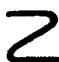
\includegraphics[keepaspectratio]{images/part001_587db9d1.jpg}}

